\begin{center}
\textbf{ \Large{Executive Summary} }
\end{center}

The Intensity Frontier (I.F.) group of the University of Texas at Arlington started in 2014 with 0.5 FTE of PI Jaehoon Yu and of PI Amir Farbin aiming for a balanced program between US-based and non-US based experiments. In order to continue to build a strong I.F. program, the group recently hired a full time I.F. junior faculty, Dr. Jonathan Asaadi. While PI Farbin has decided to transition back to the Energy Frontier (E.F), the overall strength of the group has grown to two full PI's with the successful transition of PI Yu to full time I.F.

Beyond the addition of a new faculty member, the UTA I.F. group has made significant contributions to the LArIAT, LBNE/DUNE, and MiniBooNE Experiments. Farbin played a key role of deputy computing coordinator for the DUNE project and Yu has served as a co-convener for the LBNE R$\&$D Coordination group. Yu's role has now become a co-convenership of the DUNE Beyond the Standard Model physics group beginning September 2015. UTA was also the host of the first off-Fermilab-site DUNE collaboration meeting in January, 2016, in which over 150 collaborators participated. Farbin and Yu have been supervising a student who has been contributing to the beam-dump dark matter search with first results expected Fall 2016. Asaadi has continued his roles on MicroBooNE, serving as the convener of the Astro-Particle and Exotics group through August 2016 and a lead TPC-Expert for the experiment. Asaadi has also played a leadership role on LArIAT serving as the analysis coordinator in 2015 and 2016 leading to the first measurement of the $\pi^{-}$-Argon cross-section and now will transition to serve as co-spokesperson (starting Fall 2016). The UTA group has also joined SBND (through Asaadi's existing affiliation) and the ICARUS experiment (with Yu as institutional board member) and has been contributing to the refurbishment of the light detection system with the hire of a new post-doctoral researcher (and an existing ICARUS collaborator), Dr. Andrea Falcone.

In this document, we propose to complete the ongoing effort on MiniBooNE (Yu), and continue/add significant contributions to SBND (Asaadi, Yu), MicroBooNE (Asaadi), ICARUS (Asaadi, Yu) and the Deep Underground Neutrino Experiment, DUNE (Asaadi, Yu) with a vital contribution to protoDUNE. These experiments are carefully selected to leverage our groups growing technical and analysis expertise utilizing liquid argon time projection chambers. Moreover, in order to accomplish the work laid out in this proposal, the UTA group will leverage Asaadi's start-up to provide an additional (beyond what is requested here) post-doctoral researcher (Dr. Andrea Falcone) in year one and two of this proposal. Dr. Falcone will play a leadership role on the ICARUS and SBND experiments during construction, installation and commissioning, moving to Fermilab in time with the transfer of the refurbished ICARUS detector.

The work on MiniBooNE is limited to data analysis from the beam dump data taken in 2014 for a low mass dark matter search. This is anticipated to complete shortly with the graduation of Sepideh Shahsavarani, Farbin’s Ph.D. student. This student will stay on the I.F. program for another two years till she completes her Ph.D. under the joint advisement of Farbin, Yu, and Asaadi and is expected to contribute to the other I.F. efforts. Concurrently, a second graduate student (Zack Williams) will be funded via Asaadi's start-up to allow for a transition of research duties upon Shahsavarani's graduation. Asaadi will continue to play a leadership role on LArIAT with Yu continuing support via data analysis and operations with the expected winding down of the project in the next 1-2 years.

\begin{center}
\textbf{ \Large{UTA Strategic Plan} }
\end{center} 

The UTA group will have contributions and responsibilities across the Fermilab the short-baseline neutrino (SBN) program as well as the long-baseline neutrino (LBN) program. A primary goal of the group throughout the period of this proposal is to contribute to the success of the construction and execution of these experiments. We aim to position ourselves to make major contributions to the DUNE project by playing leadership roles in the design and construction of the single and dual phase prototype detectors at CERN neutrino platform. This work is intended to allow UTA to be a world leading institution for the construction and data analysis of the DUNE detector. Synergistic with this goal, our active participation in the construction, commissioning and operation of the SBN experiments: MicroBooNE, SBND, and ICARUS allow us to enhance our expertise in LArTPC technology and produce valuable physics results, and gain experience in near/far oscillation analyses utilizing the data from these detectors.

Among the various topics described below, we consider protoDUNE to be under the most restrictive timeline and deserve immediate  attention early in the period of this renewal proposal.  This is primarily due to protoDUNEs' data taking schedule. Since the availability of charged particle beams at CERN's neutrino platform are dictated by the CERN accelerator complex upgrade schedule, having the protoDUNE detectors ready before the shutdown of the CERN accelerators at the end of 2018 is critical. Moreover, the protoDUNE projects are on the critical path for the success of the U.S. flagship experiment, DUNE. The SBN experiments are also seen by the UTA group as a high priority, but given that Fermilab will continue provide beams to these experiments through at least 2021, the impact of any delays in the construction and operation of the two future experiments is less critical.

\begin{figure}[htb]
\centering
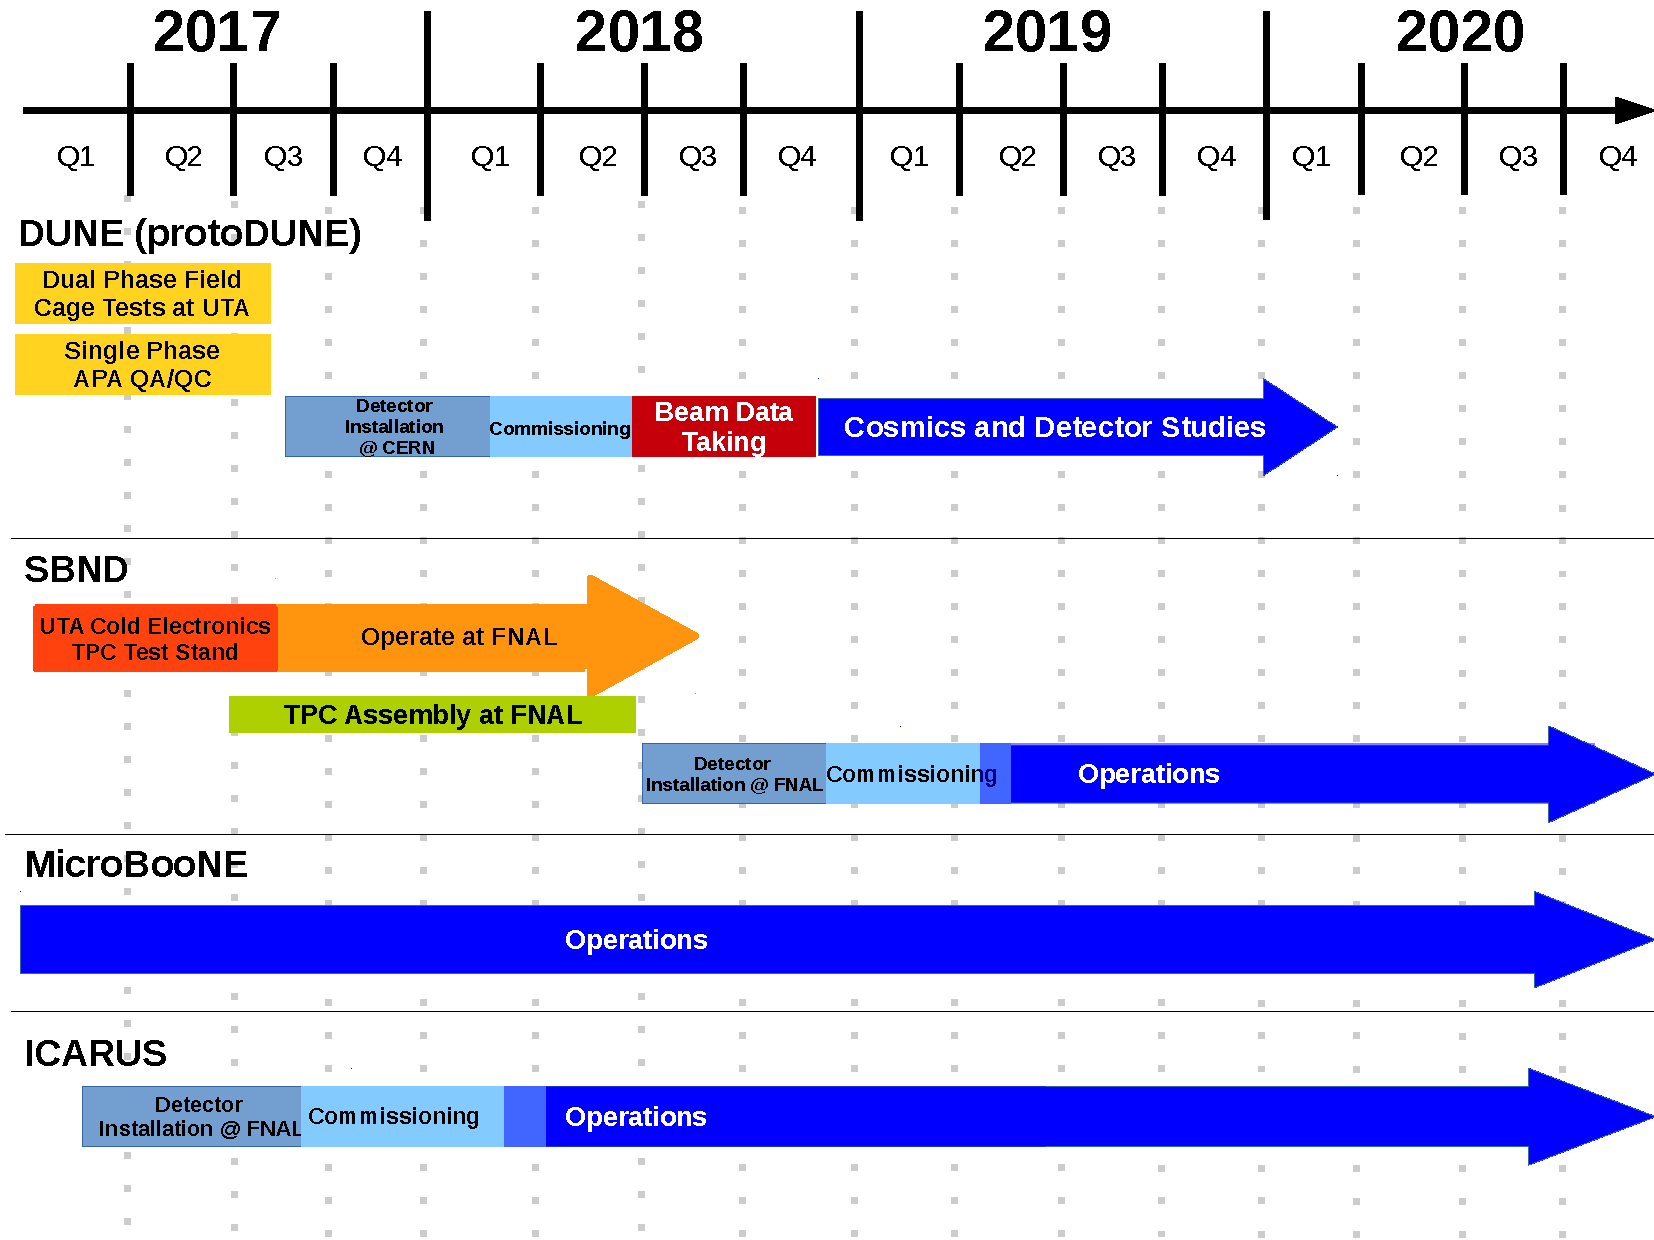
\includegraphics[width=0.80\textwidth]{images/Timeline.pdf}
\caption[]{Timeline of the strategic projects proposed .}
\label{fig:IFTimeline}
\end{figure}

Figure \ref{fig:IFTimeline} along with Tables \ref{tab:IFProjects} and \ref{tab:People} attempt to summarize the timeline, projects, and associated personnel resources that will execute the research described in greater detail in the subsequent sections. The strategic goal is to have Asaadi focus on the short and mid-term experiments such as MicroBooNE and SBND with a smaller portion of his time on ICARUS and DUNE initially and then ramping this effort over time. Meanwhile, Yu will focus on the long and mid-term experiments such as DUNE and ICARUS with a gradually increasing portion over time on the whole SBN program. This will allow our group to maintain a constant level of contribution from both the PI's and the post-doctoral and graduate researchers on all four experiments.


%%%%%%%%%%%%%%%%%%%%%%%%%%%%%%%%%%%%%%%%%%%%%%%%%%%%%%%%%%%%%%%%
\begin{center}
\begin{table}[htb]
	\begin{center}
	\resizebox{0.95\textwidth}{!}{%
	\begin{tabular}{c|c|c|c}
	\multicolumn{4}{c}{\textbf{IF Summary of Proposed Work}} \\
	\hline \hline
	\textbf{Experiment} & \textbf{Project} & \textbf{Location} & \textbf{Lead PI} \\
	\hline
	     & protoDUNE SP-APA QA/QC and installation & UTA/CERN & Asaadi \\
	DUNE & BSM Physics & UTA & Yu \\
	     & protoDUNE DP-FC Construction & UTA/CERN & Yu \\
	\hline
	     & Cold Electronics TPC Test-stand & UTA/FNAL & Asaadi \\
    SBND & Detector Construction, Installation, and Commissioning & FNAL & Yu \\	     
	     & Cross-Section Data Analysis & UTA/FNAL & Asaadi \\
	     
	\hline
	MicroBooNE & TPC Detector Expert & UTA/FNAL & Asaadi \\
	           & Detector Operations & UTA/FNAL & Asaadi \\
	           & Cross-Section Data Analysis & UTA/FNAL & Asaadi \\
	\hline
	ICARUS     & Detector Installation and Commissioning & FNAL & Asaadi \\
	           & NuMI Off-Axis Cross-Sections & UTA/FNAL & Yu \\
	           
	\hline

	MiniBooNE & Beam Dump Dark Matter Search & UTA/FNAL & Yu \\
	\hline                      
	\end{tabular}}
	\caption{Overview of the UTA projects across the Intensity Frontier} \label{tab:IFProjects}
	\end{center}
\end{table}
\end{center}
%%%%%%%%%%%%%%%%%%%%%%%%%%%%%%%%%%%%%%%%%%%%%%%%%%%%%%%%%%%%%%%%


%%%%%%%%%%%%%%%%%%%%%%%%%%%%%%%%%%%%%%%%%%%%%%%%%%%%%%%%%%%%%%%%
\begin{table}[htb]
	\begin{center}
	\resizebox{\textwidth}{!}{%
	\begin{tabular}{c|c|c|c}
	\multicolumn{4}{c}{\textbf{Summary of PI, Postdoc, and Graduate Personal}} \\
	\hline \hline
	 \textbf{Personnel} & \textbf{Associated Task} & \textbf{Years Supported} & \textbf{Source of Support}   \\
	\hline
	%%%% PostDoc #1 %%%%%
	Postdoc 1 (Animesh Chatterjee) & protoDUNE SP/DP  & 2017 - 2020 & UTA Base Grant \\
	 & SBND Operations and Data Analysis & & \\
	 & ICARUS Operations and Data Analysis & & \\
	\hline
	%%%% PostDoc #2 %%%%%
	& protoDUNE SP/DP & 2017 - 2020 & UTA Base Grant \\
	Posdoc 2 (TBN) & MicroBooNE Operations and Data Analysis & & \\
	 & SBND Cold Electronics Test Stand & & \\
	\hline
	%%%% PostDoc #3 %%%%%
	Postdoc${*}$ (Andrea Falcone) & ICARUS/SBND Installation and Commissioning  & 2017 - 2019 & UTA Start-up funds \\
	  & MicroBooNE Operations and Data Analysis  & & \\
	\hline
	%%% Grad Student 1 %%%
	Graduate Student 1(Garrett Brown) & protoDUNE SP/DP & 2017 - 2020 & UTA Base Grant \\
	  & SBND/ICARUS Operations and Data Analysis & & \\
	\hline
	Graduate Student 2a(Sepideh Shahsavarani) & MiniBooNE Data Analysis & 2017 - 2019 & UTA Base Grant \\
	& protoDUNE DP  & & \\
	\hline
	Graduate Student 2b $^{*}$ (Zack Williams) & SBND Cold Electronics Test Stand, & 2017 - 2019 & UTA Start-up funds \\
	& SBND Construction, Installation, and Commissioning  & 2019 - 2020 & UTA Base Grant \\
	 & MicroBooNE Operations and Data Analysis & & \\
	\hline
	Prof. Jonathan Asaadi & SBN/DUNE & 2017 - 2020 & UTA Base Grant \\
	 \hline
	Prof. Jae Yu & DUNE/SBN & 2017 - 2020 & UTA Base Grant \\
	 \hline
	\end{tabular}}
	\caption{Table summarizing the personnel working on the project described in this proposal. Note: Personnel marked with ``*'' denote their effort is supported for some phase of the project utilizing start-up funds. This is done to maximally leverage the UTA group across both DUNE and the SBN program.} \label{tab:People}
	\end{center}
\end{table}
%%%%%%%%%%%%%%%%%%%%%%%%%%%%%%%%%%%%%%%%%%%%%%%%%%%%%%%%%%%%%%%%


\begin{center}
\underline{\textbf{Deep Underground Neutrino Experiment (DUNE)}}
\end{center}


\noindent DUNE aims to address the questions of the neutrino mass hierarchy and CP-violation in the lepton sector by measuring the asymmetry between appearance of electron neutrinos from a beam of muon neutrinos ($P(\nu_{\mu} \rightarrow \nu_{e}$)) compared to the appearance of electron antineutrinos from a beam of muon antineutrinos and $P(\bar{\nu}_{\mu} \rightarrow \bar{\nu}_{e}$)) as well as the precise measurement of the $\nu_{e}$ energy spectrum measured at the far detector. The UTA group aims to play a major role in this U.S. flagship experiment and will contribute in the immidate future via a series of detector prototypes.


%%%%%%%%%%%%%%%%% DUNE %%%%%%%%%%%%%%%%%%%%%
\begin{itemize}
\item {{\bf protoDUNE:} The UTA group will be contributing to both the protoDUNE Dual Phase (DP) and Single Phase (SP) detectors. Asaadi and Yu expect to play a major role in various detector component construction, installation, and commissioning as well as data taking during the first years of this proposal. This work will lay the foundation to contributing to the larger DUNE project.}

\begin{itemize}
\item {{\bf ProtoDUNE SP-APA QA/QC:} Given that the highest priority of DUNE is to establish and demonstrate the functionality of its baseline technology, namely the single phase LArTPC, Asaadi will be focusing on the quality assurance, quality control, and commissioning of the anode plane assemblies (APA's) for protoDUNE SP. This work is expected to build up infrastructure, expertise, and capability to contribute and lead during the DUNE SP far detector construction.}

\item {{\bf ProtoDUNE DP-FC :} Yu will be working on design, construction and installation of the field cage (FC) for ProtoDUNE Dual Phase (DP) Detector. While the dual phase technology for DUNE is an alternative choice of the technology, the design of the field cage for ProtoDUNE DP shares a large fraction of its design with the single phase. The material, the shape of the FC loop, the use of straight unlinked FC loop, and the resistor dividor chain are examples of common aspects between the two technologies.  UTA will participating in the design, construction and installation of ProtoDUNE DP FC and position our group to build up necessary infrastructure and expertise to participate in the FC construction of both SP and DP technologies for the DUNE far detector.  We also consider the success of this project and the participation of U.S. groups to DP technology essential not only in preparing for the construction of first and second 10kt DUNE modules but also in playing an important diplomatic role in keeping the truly international character of the collaboration.}

\end{itemize}

\item {{\bf DUNE Beyond the Standard Model Physics:} UTA has been a leading participant in searching for low mass dark matter in high intensity proton beams from the start of the I.F. group in 2014. For this work, Yu has been leading the BSM physics working group of DUNE since September 2015 and has grown the group to play a significant role within the collaboration. Yu plans on ensuring various BSM topics will be part of the DUNE Technical Design Report to be released in summer 2019.}

\end{itemize}

%%%%%%%%%%%%%%%%% SBN %%%%%%%%%%%%%%%%%%%%%
\begin{center}
\underline{\textbf{The Short Baseline Neutrino (SBN) Program}}
\end{center}

\noindent The SBN program aims to conclusively address the experimental hints of sterile neutrinos through the utilization of three LArTPC detectors. An essential component for our group is to continually be producing physics results throughout the construction period of DUNE experiment and contributing to the development of LArTPC technology. In this regard, the SBN program at Fermilab provides the perfect mix short and mid-term projects for our group to continue producing new physics results and train young physicists for the future.


\begin{itemize}

%%%%%%%%%% SBND %%%%%%%%%%%%%%%%%
\item {{\bf SBND:} Given the large overlap of the collaborators between MicroBooNE and SBND, Asaadi is well recognized in the collaboration.  Therefore, Asaadi will be the institutional representative to the collaboration and lead the effort on SBND.  Yu is in discussions with the SBND management for his joining to the collaboration prior to the start of this funding period in 2017 and will contribute to the efforts outlined below and presented in greater detail in Section 3.1. } 
\begin{itemize}
\item{\textbf{Cold Electronics TPC Test-stand}}

\item{\textbf{Detector Construction, Installation, and Commissioning}}

\item{\textbf{Cross-Section Data Analysis}}

\end{itemize}

%%%%%%%%%% MicroBooNE %%%%%%%%%%%%%%
\item{{\bf MicroBooNE:} Asaadi has been an essential member of the construction, commissioning, operation and data analysis on MicroBooNE. With Asaadi being a young-tenure track faculty member, it is essential for him to be able to produce physics results in the first years of the proposal. Given this, Asaadi will focus on operations and data analysis outlined below and presented in greater detail in Section 3.2}

\begin{itemize}
\item{\textbf{Cross-section Data Analysis}}
\item{\textbf{Detector Operations}}
\item{\textbf{TPC Detector Expert}}

\end{itemize}


%%%%%%%%%% ICARUS %%%%%%%%%%%%%%
\item{{\bf ICARUS:} With the inclusion of the ICARUS experiment, this completes the short-baseline neutrino oscillation experiment utilizing a low energy neutrino beam. For this reason, the UTA group deems the success of ICARUS as an essential component of the SBN. In line with that, our group has joined the experiment as a member with Yu as the institutional board representative as one of the handful of U.S. groups to participate in it. Moreover, we have been utilizing Asaadi's start-up funds to support a post-doctoral researcher to help lead the refurbishment and integration of ICARUS. During the funding period here our efforts include the following, presented in greater detail in Section 3.3.}

\begin{itemize}
\item{\textbf{Installation and Commissioning}}
\item{\textbf{Detector Operations}}
\item{\textbf{NuMI Off-Axis Cross-Sections}}

\end{itemize}

\end{itemize}


With this strategic plan in place, the activities proposed aim to ensure synergy between the SBN and LBN efforts and optimize our use of resources. What follows is a broad introduction to the compelling physics which motivates this research program as well as a more detailed sketch of the program of work which is intended to be executed in the intensity frontier.

\subsection{Physics Introduction}
The discovery that neutrinos undergo oscillation in their flavor, and thus are massive particles, serves as one of the first pieces of evidence for physics beyond the Standard Model (SM) of particle physics. The prevailing description of neutrino oscillations provided by the Pontecorvo-Maki-Nakagawa-Sakata (PMNS) matrix characterizes the flavor change as a result that the neutrino flavor eigenstates ($\nu_{e}, \nu_{\mu}, \nu_{\tau}$) are a linear combination of the neutrino mass eigenstates ($\nu_{1}, \nu_{2}, \nu_{3}$). The rotation from the mass eigenstates to the flavor eigenstates is governed by three angles $\theta_{i,j}$, where $i$ and $j$ correspond to the mass eigenstates with $i < j$, and a phase $\delta$ which determines magnitude of charge-parity (CP) violation within the neutrino sector. In addition, the flavor change of the neutrinos depends on the ratio of neutrino energy and the distance traveled by the neutrino (often referred to as the baseline) as well as the difference in the square of the mass eigenstates $\Delta m_{ji}^{2}$. Neutrinos produced in the atmosphere \cite{No1, No2, No3}, in nuclear reactors \cite{No4, No5, No6}, in the sun \cite{No7, No8, No9}, as well as in man-made particle accelerators \cite{No10, No11, No12} have been used to study the phenomenon of neutrino oscillations. The exact ordering of the neutrino mass states, known as the mass hierarchy, as well as the size of the CP-violating phase $\delta$ are, as yet, unknown. These quantities remain one of the last major pieces of the Standard Model of particle physics and offer the opportunity to answer such fundamental questions as:

\begin{itemize}
\item[1)] \textbf{What is the origin of the matter/antimatter asymmetry in the universe?}

\item[2)] \textbf{Do we understand the fundamental symmetries of the universe?}

\item[3)] \textbf{Is the three-flavor paradigm of the Standard Model for neutrino oscillation the accurate description for neutrino interactions?}
\end{itemize}

Into this experimental landscape, there exists a set of series of experimental measurements which suggest that the three-flavor paradigm of neutrino oscillations is incomplete. Two general classes of anomalous observations may point to additional physics beyond the SM  in the neutrino sector.

\begin{itemize}
\item \textbf{The disappearance signal in low energy electron anti-neutrinos from reactor neutrino experiments \cite{No13} \textit{(``Reactor Neutrino Anomaly'')} and Mega-Curie radioactive electron neutrino sources in Gallium \cite{No14, No15} \textit{(``Gallium Anomaly'')}}

\item \textbf{The electron-like excess from muon neutrino (and anti-neutrino) particle accelerators \textit{(``LSND/MiniBooNE Anomaly'')} \cite{No16, No17}}

\end{itemize}

Neither of these anomalies can be accounted for by the standard three-flavor oscillations of the SM and may hint at the existence of additional neutrino states with larger mass difference ($\Delta m_{new}^{2}\geq 0.1 eV^{2}$) which participate in the mixing of the flavour states (referred to as ``sterile neutrinos''). Definitive evidence of the existence of new neutrino states would be a revolutionary discovery with broad implications for both particle physics and cosmology. Moreover, in order for future accelerator based neutrino experiments to disentangle the mass hierarchy and search for CP-violation, the oscillation framework must be concretely known and precisely measured.

Liquid Argon Time Projection Chambers (LArTPCs) offer fine-grain tracking as well as powerful calorimetry and particle identification capabilities making them ideal detectors for studying neutrino-nuclei interactions. When a neutrino interacts with an atom in the liquid argon multiple final state charged particles as well as electromagnetic objects (such as photons and electrons) can be produced. When the charged particles traverse the liquid argon they produce ionization which drifts along the electric field inside the TPC towards a set of wire planes which are oriented at different angles with respect to each other. The drifting ions produce an electric signal on the wire planes, which is read out of the detector. By knowing the drift speed of the ions and the timing of the interaction as well as the deposition of charge on the wires a three-dimensional image of the interaction can be reconstructed. The information of the charge deposition in addition to the topological information allows for particle identification and calorimetric reconstruction. This allows, for example, the ability to disentangle electron initiated electromagnetic showers from photon initiated showers by looking at the displacement in the start of the electromagnetic shower from a primary vertex as well as analyzing the energy deposited in the first centimetres of the shower (dE/dX), shown schematically in Fig. \ref{fig:LArTPC}.

\begin{figure}[htb]
\centering
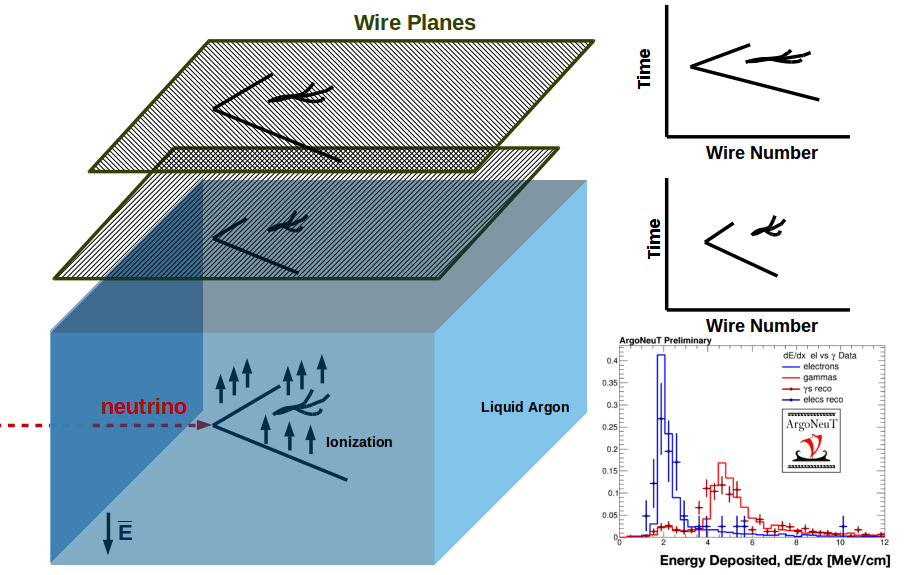
\includegraphics[width=0.55\textwidth]{images/lartpc.png}
\caption[]{Operating principals of LArTPC detectors.}
\label{fig:LArTPC}
\end{figure}

For these reasons, this detector technology has been chosen for both the study of neutrino oscillations over relatively short baselines ($<1$~km) and long baselines ($>1000$~km). The combination of millimeter scale tracking capabilities, outstanding calorimetry through a fully active/sampling detector, and powerful particle identification made by combining the ionization along the particle trajectory (dE/dX) and the topological information, have made LArTPCs the premier neutrino detector technology choice for the future.  This common neutrino detector technology is at the center point of the physics program the UTA I.F. group is aiming to utilize to explore this physics landscape and attempt help answer these fundamental questions.




